% ============================================================
% main.tex — the handout itself
%
% This file is structure and content. Every typographic
% decision lives in handoutstyle.sty.
%
% Compile with LuaLaTeX, not pdflatex:
%   latexmk -lualatex main
% ============================================================


\documentclass[11pt]{article}


% ============================================================
% LOAD HANDOUT STYLE
%
% With [unnumbered] the sections lose their numbers, and
% exercises and theorems count flat through the document:
% Exercise 1, 2, 3 instead of 1.1, 1.2. Suits a handout
% about a single topic.
% ============================================================
\usepackage{handoutstyle}
% \usepackage[unnumbered]{handoutstyle}


% ============================================================
% LANGUAGE
% ============================================================
\usepackage[english]{babel}


% ============================================================
% OPTIONAL HANDOUT TWEAKS  (uncomment to enable)
% ============================================================

% --- No paragraph indentation ---
% Use parskip, not a bare \parindent=0pt: the style also zeroes
% \parskip, so parindent alone leaves paragraphs with no separation.
% \usepackage{parskip}

% --- No page numbers (needs BOTH lines) ---
% \maketitle forces "plain" on page 1, so also uncomment the
% \thispagestyle{empty} after \maketitle to clear the number there.
% \pagestyle{empty}


% ============================================================
% CUSTOM PACKAGES
%
% Add project-specific packages here.
% Do not insert packages elsewhere in the file.
% ============================================================

% --- Mathematics (defaults) ---
\usepackage{amsmath}                % no amssymb: unicode-math
                                    % supplies the symbols
% mathtools is NOT loaded -- see the README for the
% unicode-math-native alternatives

% --- Vectors: \vv{F}, a flat arrow that spans the whole symbol ---
% The size fix esvect needs under unicode-math lives in the style
% file, guarded so it activates only when the package is loaded.
\usepackage[e]{esvect}

% --- Units: \qty{9.81}{\metre\per\second\squared} ---
\usepackage{siunitx}
\sisetup{per-mode=symbol, separate-uncertainty=true}

% --- Tensor indices: \tensor{R}{^\rho_\sigma_\mu_\nu} ---
\usepackage{tensor}

% --- Bra-ket: \bra{\psi}, \ket{\phi}, \braket{\psi}{\phi} ---
\usepackage{physics2}
\usephysicsmodule{braket}

% The old `physics` package is not used here: it is unmaintained and
% written for the pdflatex era. It does still work alongside siunitx if
% you add \AtBeginDocument{\RenewCommandCopy\qty\SI}, at the cost of one
% siunitx warning -- but physics2 covers the same ground without it.

% --- Figures ---
\usepackage{graphicx}                % figures
\graphicspath{{figures/}}            % figures live in figures/

% --- Other ---
\usepackage{tikz}                   % native TikZ figures


% ============================================================
% CUSTOM COMMANDS
%
% Project-specific macros.
%
% The \separator rule is provided by handoutstyle.sty.
% ============================================================

% Upright d and i: \symup is the unicode-math form (\mathrm also works).
% \newcommand{\dd}{\symup{d}}
% \newcommand{\ii}{\symup{i}}
% \newcommand{\dv}[2]{\frac{\dd #1}{\dd #2}}
% \newcommand{\pdv}[2]{\frac{\partial #1}{\partial #2}}


% ============================================================
% METADATA
% ============================================================
\title{Handout Title}
\date{Spring 2026 $\cdot$ Course Name}


% ============================================================
% DOCUMENT
% ============================================================
\begin{document}

\maketitle
% \thispagestyle{empty}   % page 1: clears the number (see \pagestyle above)


% ============================================================
% SECTION
% ============================================================
\section{Energy and Conservation}

A particle of mass $m$ moves in a one-dimensional potential
$V(x)$. The total mechanical energy is
\begin{equation}
  E = \tfrac{1}{2} m v^2 + V(x),
\end{equation}
which is conserved when no external forces act.

\begin{definition}
A force is \emph{conservative} if it can be written as the
negative gradient of a potential, $F(x) = -\,\mathrm{d}V/\mathrm{d}x$.
\end{definition}

\begin{theorem}
For a conservative force, the total mechanical energy $E$ is
constant along any solution of the equation of motion.
\end{theorem}

\begin{remark}
The converse fails in general: dissipative systems admit no
such potential, and $E$ is not conserved.
\end{remark}

\subsection{Potential Energy Diagrams}

A plot of $V(x)$ against $x$ summarizes the qualitative motion at a
glance: the particle is confined to regions where $E \ge V(x)$, and
turning points occur where $E = V(x)$, as illustrated in
Figure~\ref{fig:potential}.

% TikZ figure example: use darkorange for energy levels / structural
% elements, darkolive for curves, black for axes,
% gray for secondary labels.  darkred is reserved for
% the separator rule -- do not use it in figures.
\begin{figure}[ht]
  \centering
  \begin{tikzpicture}[>=stealth]
    % Axes
    \draw[->,thick] (-2.2,0) -- (2.2,0) node[right,font=\small] {$x$};
    \draw[->,thick] (0,-0.2) -- (0,3.5) node[above,font=\small] {$V$};
    % Parabola V(x) ~ x^2 (darkolive)
    \draw[darkolive,thick,domain=-1.85:1.85,samples=60]
      plot (\x, {\x*\x});
    \node[darkolive,right,font=\small] at (1.7,3.1) {$V(x)$};
    % Energy level (darkorange)
    \draw[darkorange,thick] (-1.6,2.56) -- (1.6,2.56);
    \node[right,font=\small,darkorange] at (1.65,2.56) {$E$};
    % Classical turning points (gray dashed)
    \draw[gray,thin,dashed] (-1.6,0) -- (-1.6,2.56);
    \draw[gray,thin,dashed] ( 1.6,0) -- ( 1.6,2.56);
    \node[below,font=\small,gray] at (-1.6,0) {$-x_0$};
    \node[below,font=\small,gray] at ( 1.6,0) {$x_0$};
  \end{tikzpicture}
  \caption{Harmonic potential (\textcolor{darkolive}{olive}) with energy
           level $E$ (\textcolor{darkorange}{orange}) and classical
           turning points $\pm x_0$ (gray).}
  \label{fig:potential}
\end{figure}

The subsection heading above sits one size step below the section
title, while remaining at body size --- enough to mark a finer level
when the handout is used for lecture notes.


% ============================================================
% EXERCISE
% ============================================================
\begin{exercise}[Simple harmonic oscillator]
Consider a particle of mass $m$ in the potential
$V(x) = \tfrac{1}{2}kx^2$.

\begin{subproblems}
  \item Write down the equation of motion using Newton's
        second law.
  \item Show that
        $E = \tfrac{1}{2}mv^2 + \tfrac{1}{2}kx^2$
        is conserved along solutions.
\end{subproblems}

The result can be verified by differentiating $E$ with respect
to time and using the equation of motion from part~(a).

\begin{subproblems}[resume]
  \item Find the angular frequency of small oscillations.
\end{subproblems}
\end{exercise}

\separator


% ============================================================
% EXERCISE
% ============================================================
\begin{exercise}[Inclined plane]
A block of mass $m$ slides down a frictionless inclined plane
that makes an angle $\theta$ with the horizontal.

\begin{subproblems}
  \item Find the acceleration along the plane.
  \item How long does it take to slide a distance $L$ from rest?
  \item What is the speed at the bottom?
\end{subproblems}
\end{exercise}


% ============================================================
% SECTION
% ============================================================
\section{Circular Motion}

\begin{figure}[t]
  \centering
  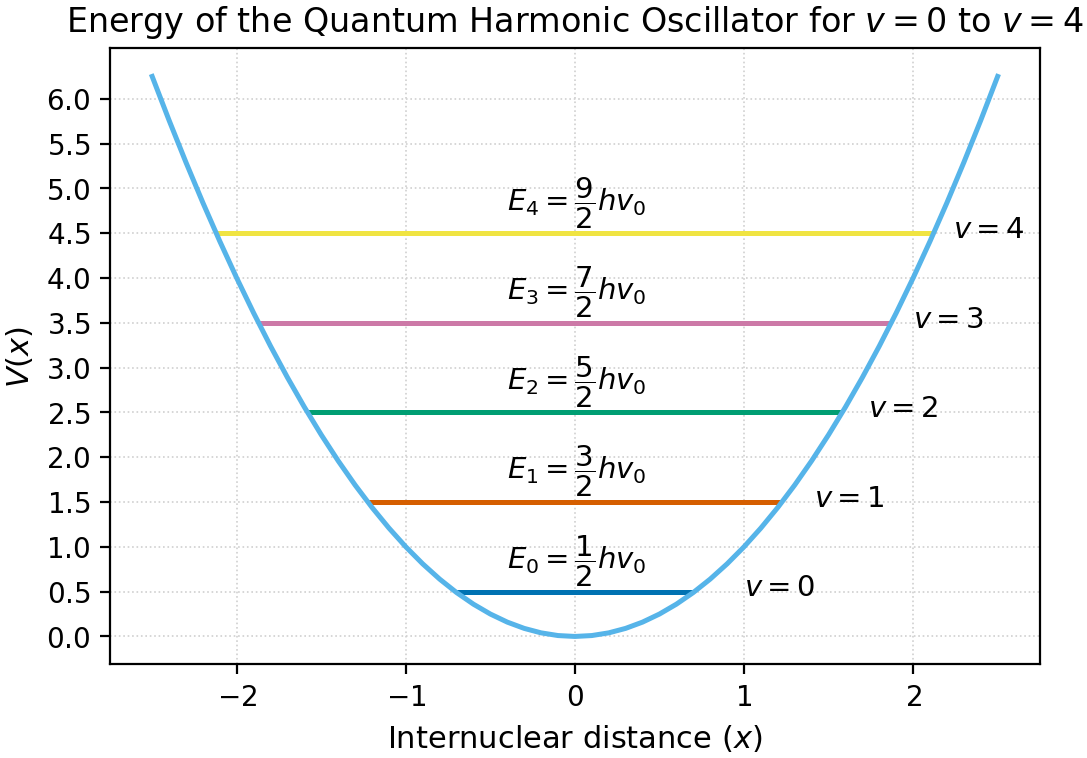
\includegraphics[width=0.5\linewidth]{Energy_levels}
  \caption{Schematic figure for the topic.}
  \label{fig:circular}
\end{figure}

In uniform circular motion, the centripetal acceleration has
magnitude $a_c = v^2/r$, directed toward the center of the
circle.


% ============================================================
% EXERCISE
% ============================================================
\begin{exercise}[Circular orbit]
\label{ex:orbit}
A satellite moves in a circular orbit at radius $r$ around a
planet of mass $M$.

\begin{subproblems}
  \item Show that the orbital speed is $v = \sqrt{GM/r}$,
        where $G$ is Newton's gravitational constant.
  \item Express the orbital period $T$ in terms of $r$, $M$,
        and $G$.
\end{subproblems}
\end{exercise}


% ============================================================
% SECTION
% ============================================================
\section{Numerical Example}

The \verb|python| environment typesets code with Gruvbox Light
syntax highlighting. The short script below verifies the orbital
speed and period from Exercise~\ref{ex:orbit} numerically for three representative
radii.

\begin{python}
import numpy as np

G = 6.674e-11   # gravitational constant  (m^3 kg^-1 s^-2)
M = 5.972e24    # Earth mass              (kg)

orbits = {"Low orbit":    6.40e6,
          "ISS (approx)": 6.78e6,
          "GEO":          4.22e7}

for name, r in orbits.items():
    v = np.sqrt(G * M / r)           # orbital speed  [m/s]
    T = 2 * np.pi * r / v / 3600    # orbital period [hours]
    print(f"{name:14s}  v = {v/1e3:.3f} km/s   T = {T:.2f} h")
\end{python}


\end{document}
